 \paragraph{} Les test ont été effectués sur des matrices 7x7 dus aux limitations de contraintes dans la version étudiant de AMPL avec le solveur knitro (300 contraintes maximum).  De ce fait, nous nous sommes limités également au premier modèle décrit dans l'article pour AMPL.

\paragraph{} Les résultats de la version mathématiques sont plus précis, mais plus lent (car la limite de contrainte nous empêche de l'optimiser). De plus, le temps augmente expentionellement avec le nombre de lampadaires tandis que l'énumération exhaustive montre une progression linéaire. Cela peut être observé sur les graphiques ci-dessous.


\begin{figure}
        \begin{minipage}{.5\textwidth}
        \subfloat[AMPL]{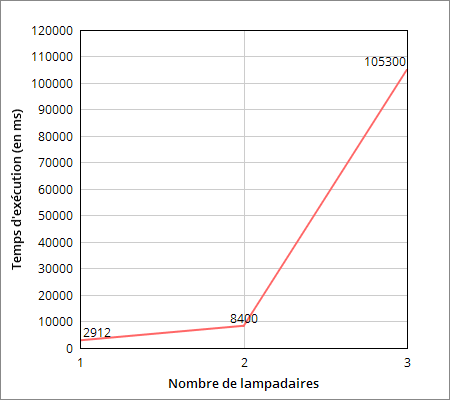
\includegraphics[scale=0.5]{./image/graphiqueAMPL.png}}
        \end{minipage}
        \begin{minipage}{.5\textwidth}
        \subfloat[Backtracking]{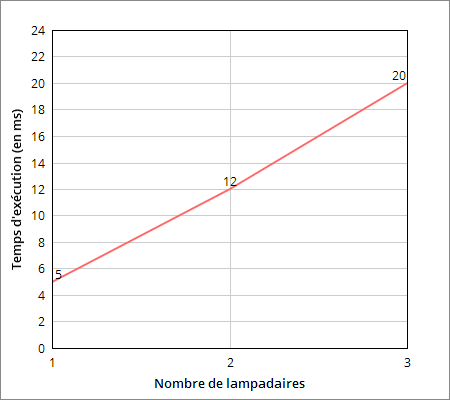
\includegraphics[scale=0.5]{./image/graphiqueBacktrack.png}}
        \end{minipage}
\end{figure}


\paragraph{} Quant aux résultats, la puissance variable permet au mieux de se rapprocher de la demande. Ici, l'on peut voir les résultats pour les 3 algorithmes.

\begin{figure}
        \begin{minipage}{.5\textwidth}
        \subfloat[Exemple de coloriage]{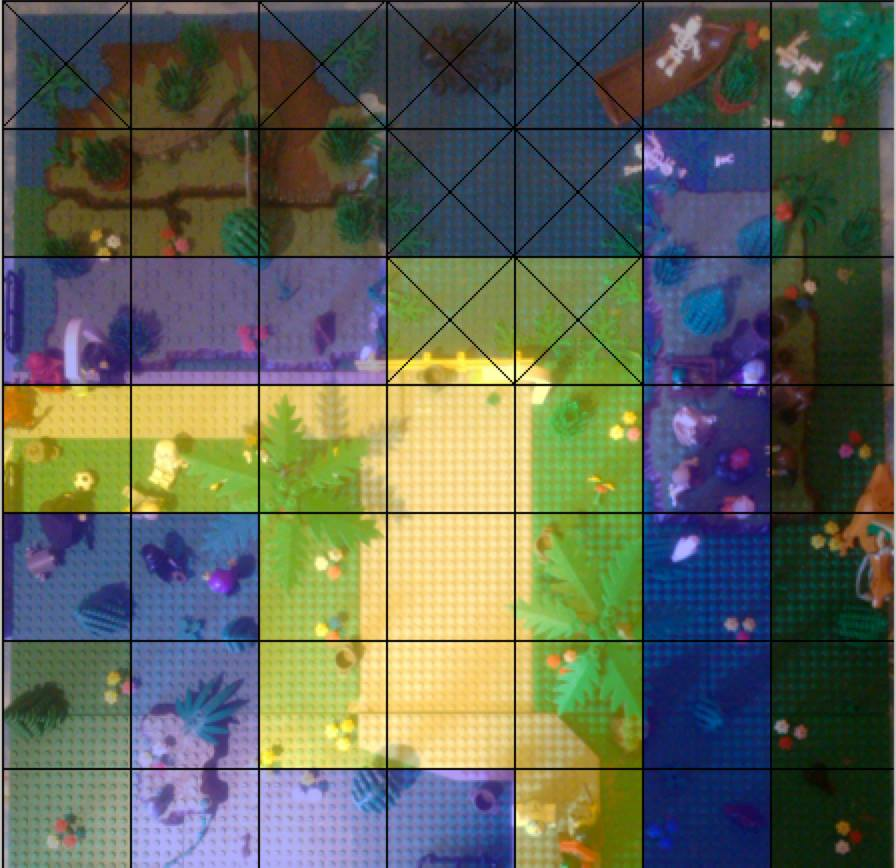
\includegraphics[scale=0.25]{./image/plateauColoriage1.jpg}}\par
         \subfloat[Résultat AMPL]{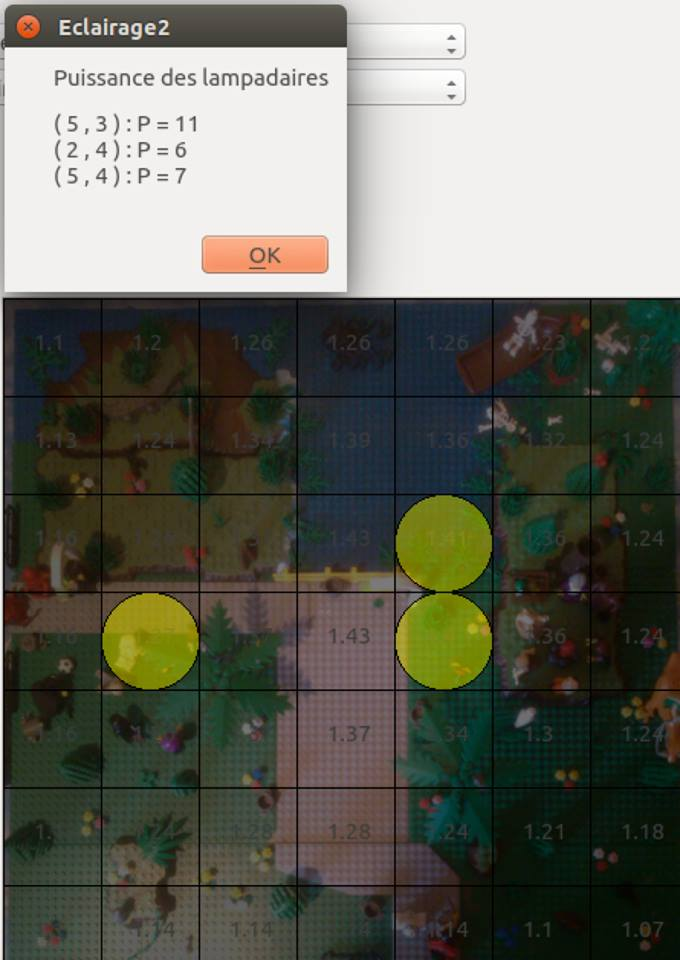
\includegraphics[scale=0.25]{./image/ampl1.jpg}}
        \end{minipage}
        \begin{minipage}{.5\textwidth}
        \subfloat[Résultat Backtracking]{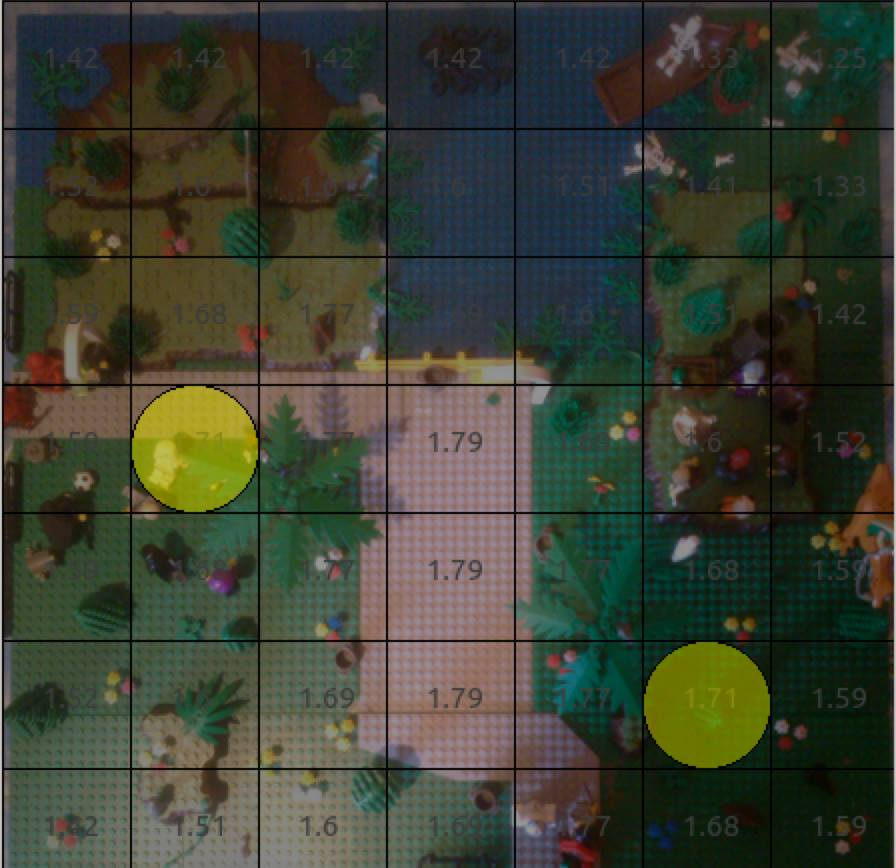
\includegraphics[scale=0.25]{./image/backtrack1.jpg}}\par
        \subfloat[Résultat Backtracking rapide]{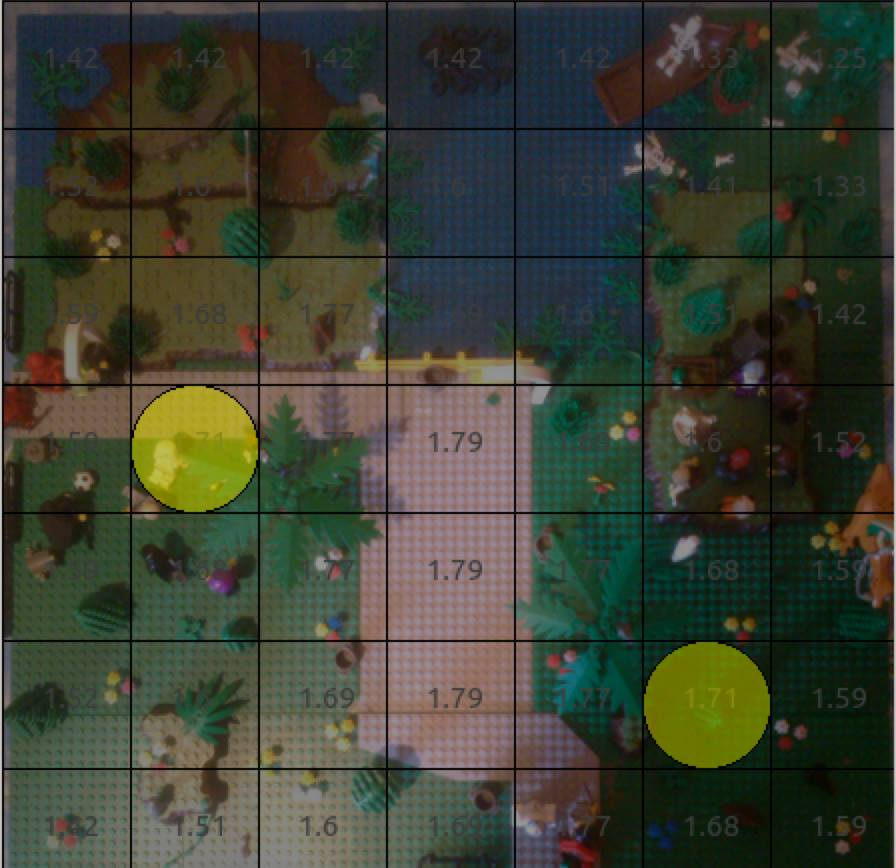
\includegraphics[scale=0.25]{./image/backtrackFast1.jpg}}
        \end{minipage}
\end{figure}

